% $Header$

\documentclass{beamer}

% This file is a solution template for:

% - Talk at a conference/colloquium.
% - Talk length is about 20min.
% - Style is ornate.



% Copyright 2004 by Till Tantau <tantau@users.sourceforge.net>.
%
% In principle, this file can be redistributed and/or modified under
% the terms of the GNU Public License, version 2.
%
% However, this file is supposed to be a template to be modified
% for your own needs. For this reason, if you use this file as a
% template and not specifically distribute it as part of a another
% package/program, I grant the extra permission to freely copy and
% modify this file as you see fit and even to delete this copyright
% notice. 


\mode<presentation>
{
  \usetheme{Warsaw}
  % or ...

  \setbeamercovered{transparent}
  % or whatever (possibly just delete it)
}


\usepackage[english]{babel}
% or whatever

\usepackage[latin1]{inputenc}
% or whatever

\usepackage{times}
\usepackage[T1]{fontenc}
% Or whatever. Note that the encoding and the font should match. If T1
% does not look nice, try deleting the line with the fontenc.
\begin{document}

\begin{frame}{Problem Identification}
What properties of a mushroom guarantee its edibility? toxicity?
\begin{enumerate}
\item Context: 
Mushroom hunting is a potentially very lucrative, but
eating the wrong mushroom can be very poisonous.
\item Criteria for success:
\begin{itemize}
\item low false positive rate (would like to keep most edible ones)
\item very low false negative rate (going to the ER would be bad)
\end{itemize}
\item Scope of solution space: Focus on mushrooms in North
America. Look at categorical data determined by the phenotype of a
mushroom, e.g. its cap, gills, etc.
\end{enumerate}
\end{frame}

\begin{frame}{Problem Identification}
\begin{enumerate}
\setcounter{enumi}{3}
\item Constraints within solution space:
\begin{itemize}
\item The data is 30 years old (may not be up to date)
\item Model may not be accurate on other continents
\end{itemize}
\item Stakeholders to provide key insight:
\begin{itemize}
\item mushroom foragers
\item mycologists
\end{itemize}
\item Key data source:

Kaggle dataset from a 30-year-old UCI Machine Learning repository
-- describes hypothetical samples corresponding to 23 species of
gilled mushrooms from The Audubon Society Field Guide to North
American Mushrooms (1981).
\end{enumerate}
\end{frame}

\begin{frame}{Recommendation and key findings}
We are able to determine the four traits most strongly associated with
poisonous mushrooms. They are, in order of importance, green spore prints
(\texttt{r}), creosote odors (\texttt{c}), narrow gills (\texttt{n}), and
silky stalk surfaces above the ring (\texttt{k}).
This agrees with the histograms in our exploratory data analysis:
\begin{center}
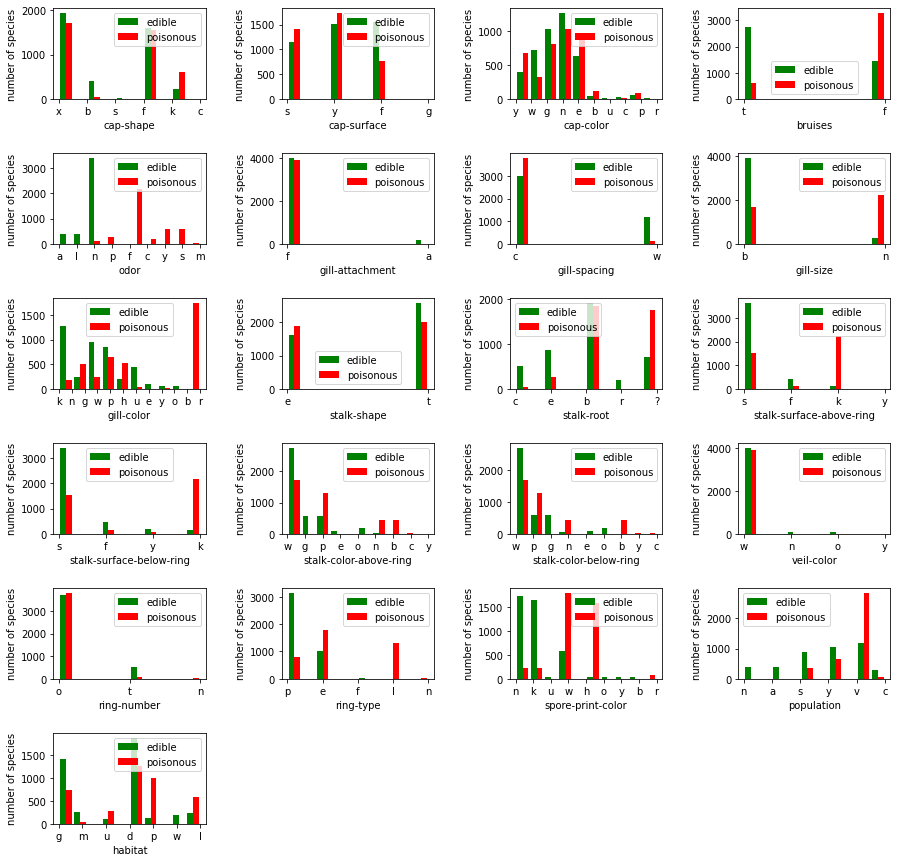
\includegraphics[scale=0.4,trim=460 150 220 570,clip=true]{histograms.png}
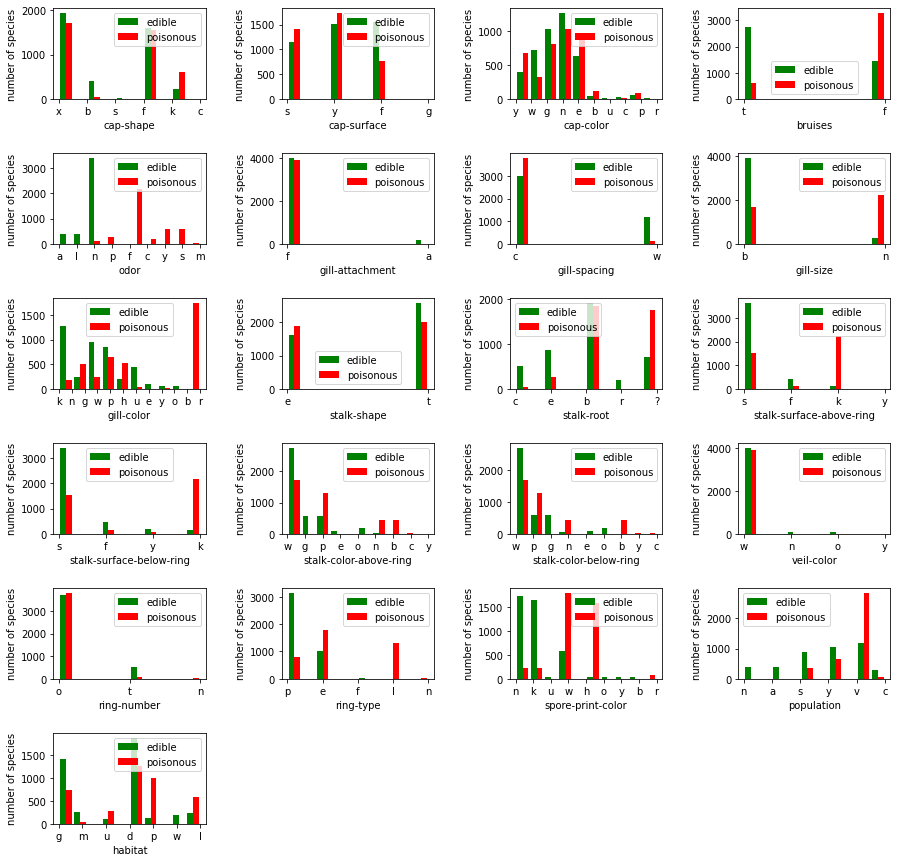
\includegraphics[scale=0.4,trim=0 585 680 135,clip=true]{histograms.png}

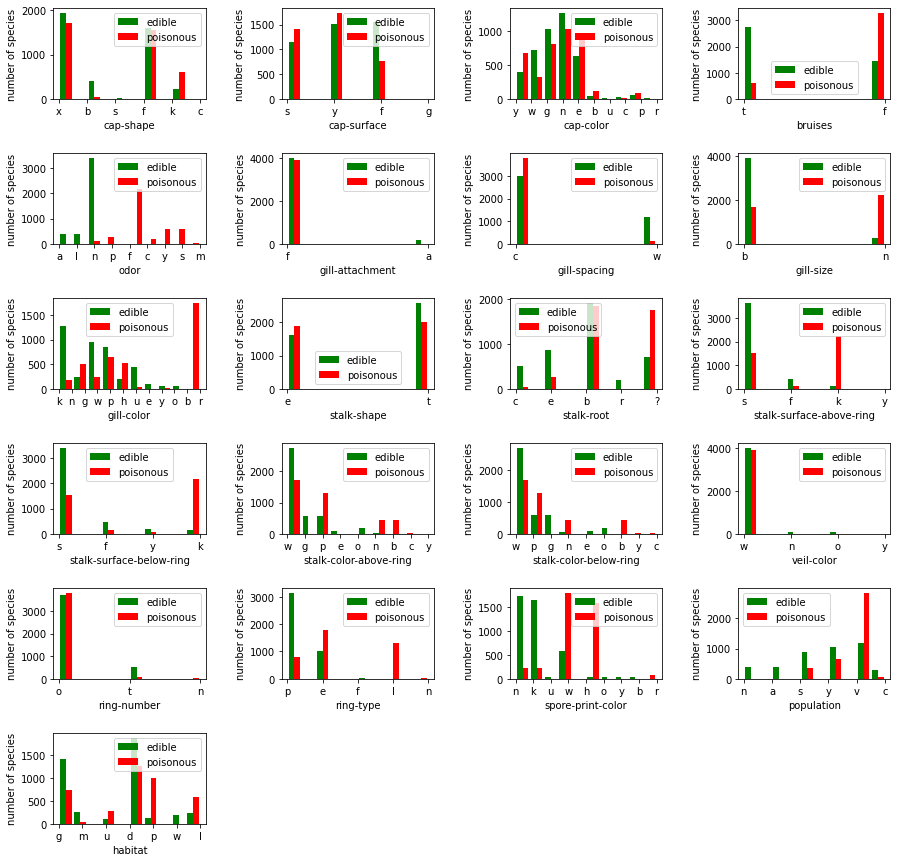
\includegraphics[scale=0.4,trim=680 575 0 145,clip=true]{histograms.png}
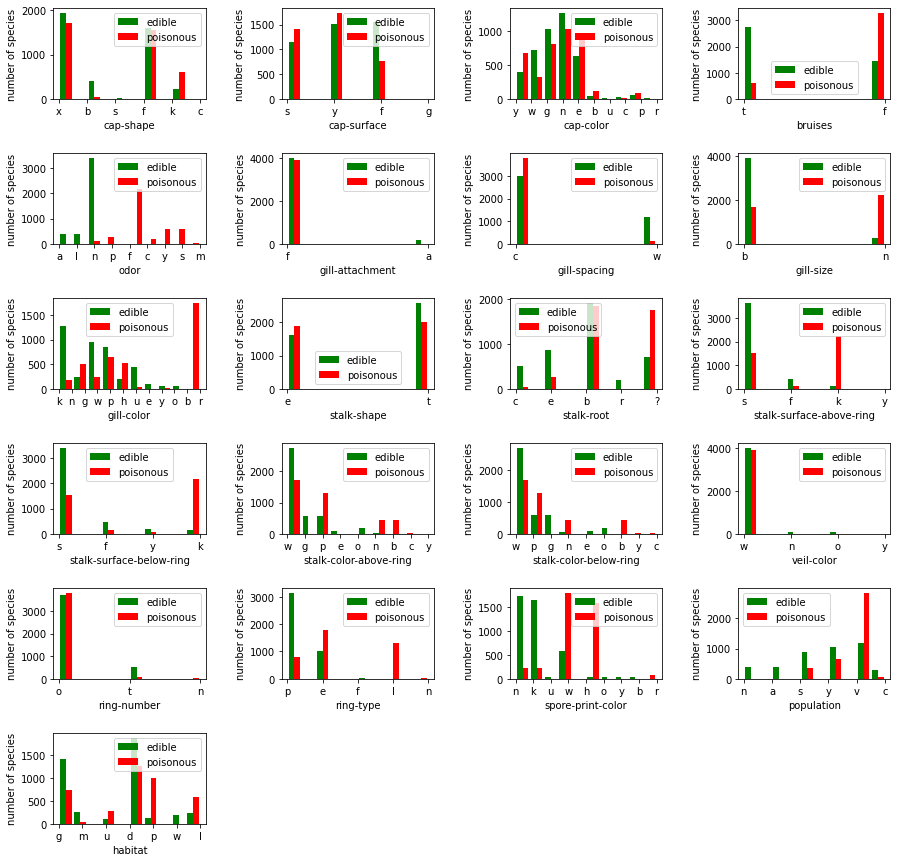
\includegraphics[scale=0.4,trim=680 430 0 280,clip=true]{histograms.png}
\end{center}
\end{frame}

\begin{frame}{Recommendation and key findings}
We are also able to determine the four traits most strongly
associated with edible mushrooms. They are, in order of importance, almond
odors (\texttt{a}), anise odors (\texttt{l}), no odors (\texttt{n}), and
crowded gill spacing (\texttt{w}).
This agrees with the histograms in our exploratory data analysis:
\begin{center}
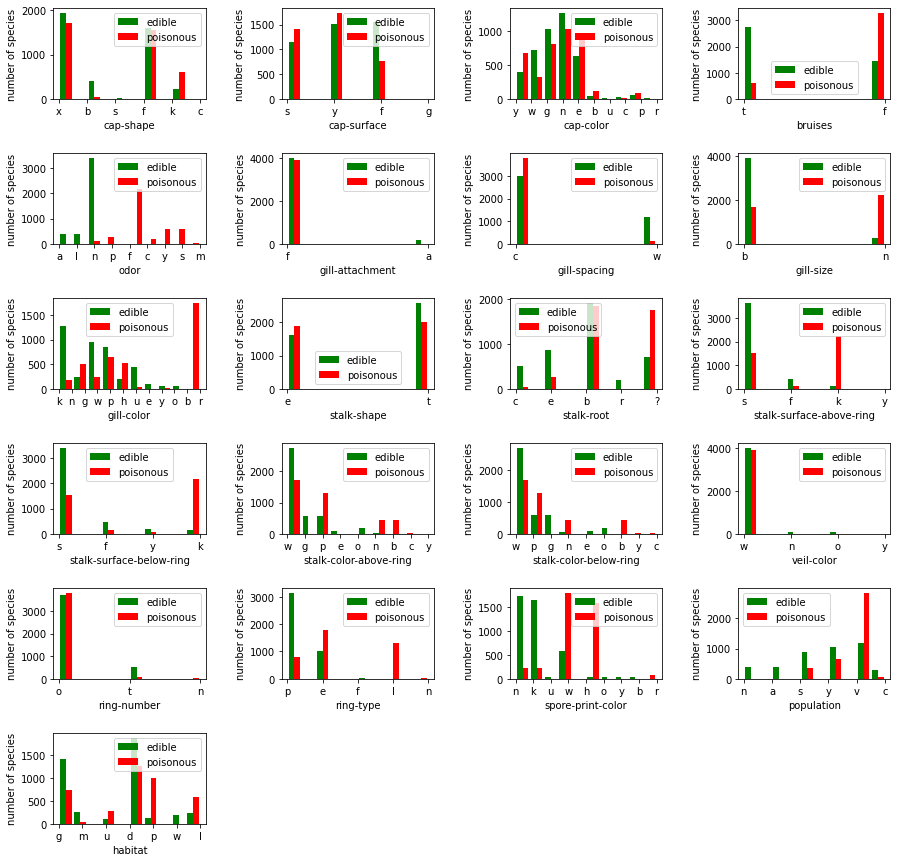
\includegraphics[scale=0.6,trim=0 575 680 145,clip=true]{histograms.png}
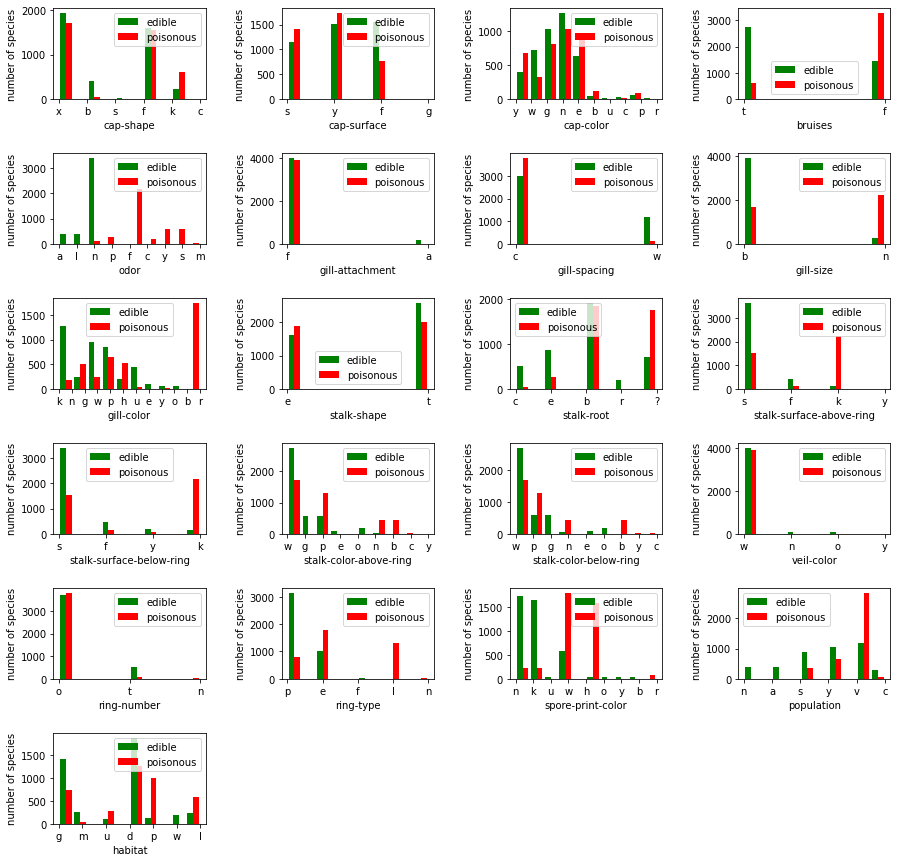
\includegraphics[scale=0.6,trim=460 575 220 145,clip=true]{histograms.png}
\end{center}
\end{frame}

\begin{frame}{Modeling results and analysis}
\begin{center}
SVC coefficients for poisonousness:
\begin{tabular}{|c|c|}\hline
\texttt{spore-print-color\_r} & $1.591870$ \\\hline
\texttt{odor\_c} & $1.045295$ \\\hline
\texttt{gill-size\_n} & $0.799876$ \\\hline
\texttt{stalk-surface-above-ring\_k} & $0.778354$ \\\hline
\texttt{population\_c} & $0.762460$ \\\hline
$\vdots$ & $\vdots$ \\\hline
\texttt{stalk-root\_r} & $-0.583111$ \\\hline
\texttt{gill-spacing\_w} & $-0.621908$ \\\hline
\texttt{odor\_n} & $-0.844349$ \\\hline
\texttt{odor\_l} & $-1.022896$ \\\hline
\texttt{odor\_a} & $-1.022902$ \\\hline
\end{tabular}
\end{center}
\end{frame}

\begin{frame}{Modeling results and analysis}
Logistic regression coefficients for poisonousness:
\begin{center}
\begin{tabular}{|c|c|}\hline
\texttt{gill-size\_n} & $3.125447$ \\\hline
\texttt{stalk-surface-above-ring\_k} & $3.101673$ \\\hline
\texttt{bruises\_t} & $2.537706$ \\\hline
\texttt{stalk-root\_c} & $1.694761$ \\\hline
\texttt{ring-type\_p} & $0.682597$ \\\hline
$\vdots$ & $\vdots$ \\\hline
\texttt{spore-print-color\_k} & $-3.908160$ \\\hline
\texttt{spore-print-color\_n} & $-3.965740$ \\\hline
\texttt{odor\_l} & $-5.063126$ \\\hline
\texttt{odor\_a} & $-5.108882$ \\\hline
\texttt{odor\_n} & $-6.226523$ \\\hline
\end{tabular}
\end{center}
\end{frame}

\begin{frame}{Modeling results and analysis}
\begin{center}
Random forest feature importances:
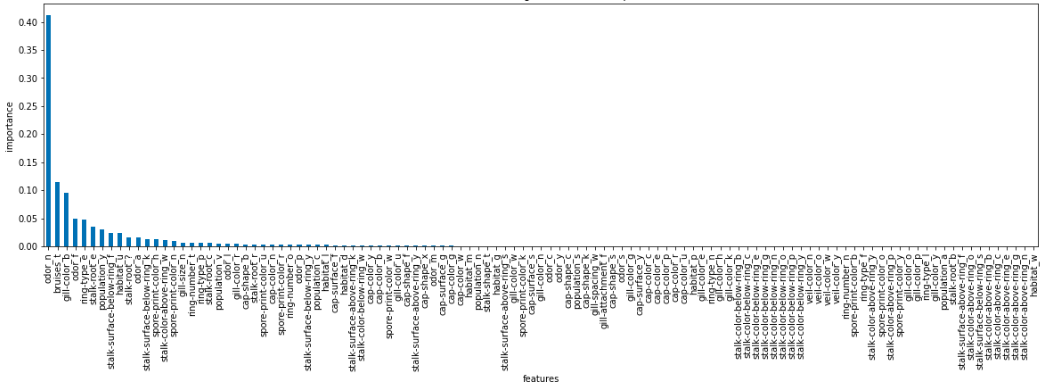
\includegraphics[scale=0.3]{random-forest-mushrooms}
\end{center}
\end{frame}

\begin{frame}{Summary and conclusion}
\begin{itemize}
\item The most poisonous mushroom features are green spore prints,
creosote odors, narrow gills, and silky stalk surfaces above the ring.

\item The features most strongly associated with edible mushrooms are almond
odors, anise odors, no odors, and crowded gill spacing.

\item Other important features determining mushroom class are bruises, buff gill
color, and club stalk roots.
\end{itemize}
\end{frame}
\end{document}
